\newpage
\subsection{Declaring classes and attributes}
\visHeader
\hypertarget{static:classes vis}{}

\begin{itemize}

\item[$\blacktriangleright$] Return to EA, and double-click your \texttt{LearningBoxLanguage} diagram to ensure it's open.

\vspace{0.5cm}

\item[$\blacktriangleright$] There are two ways for you to create your first \texttt{EClass}. First, to the left of the workbench, a \emph{Toolbox} containing
the Ecore types available for metamodelling should have appeared (Fig.~\ref{ea:eclass}).\footnote{If not, choose ``Diagram/Diagram Toolbox'' to show the
current toolbox} Click on the \texttt{EClass} icon then somewhere in the diagram to create a new object. Alternatively, you can click in the diagram and press
\texttt{space} to invoke the toolbox context menu, then select \texttt{EClass}.

\vspace{0.5cm}

\begin{figure}[htbp]
	\centering
  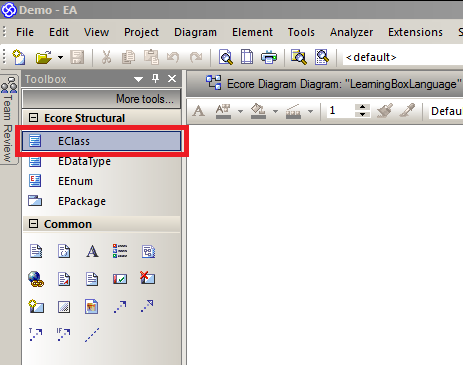
\includegraphics[width=0.7\textwidth]{ea_createEClass}
	\caption{Create an EClass}
	\label{ea:eclass}
\end{figure}

\vspace{0.5cm}

\item[$\blacktriangleright$] In the dialogue that pops-up, set \texttt{Box} as the name and click \texttt{OK} (Fig.~\ref{ea:eclass_properties}).
This dialogue can always be invoked again by double-clicking the EClass, or by pressing \texttt{alt} and single-clicking. It contains many other properties
we'll investigate later in the handbook. In general, a similar properties dialogue can be opened in the same fashion for almost every element in EA.

\clearpage

\begin{figure}[ht]
	\centering
  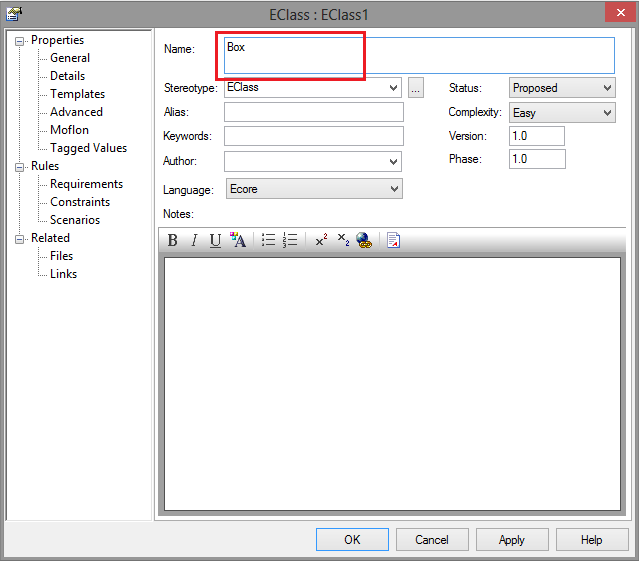
\includegraphics[width=0.8\textwidth]{ea_propertiesEClass}
	\caption{Edit the properties of an EClass}
	\label{ea:eclass_properties}
\end{figure}

\item[$\blacktriangleright$] After creating \texttt{Box}, your EA workspace should resemble Fig.~\ref{ea:eclass_completed}.

\vspace{0.5cm}

\begin{figure}[htbp]
	\centering
  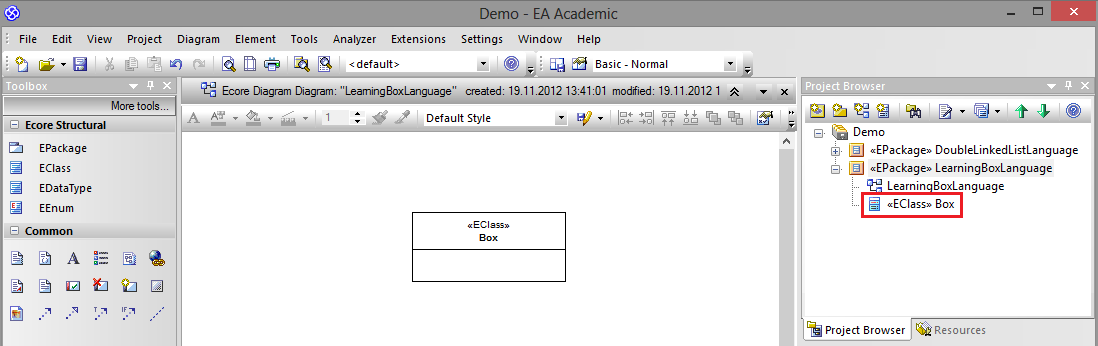
\includegraphics[width=1\textwidth]{ea_afterBoxCreation}
	\caption{State after creating \texttt{Box}}
	\label{ea:eclass_completed}
\end{figure}

\item[$\blacktriangleright$] Now create the \texttt{Partition} and \texttt{Card} EClasses the same way, until your workspace resembles
Fig.~\ref{ea:all_eclasses}. These are the main classes of your learning box metamodel.

\vspace{0.5cm}

\item[$\blacktriangleright$] Lets add some attributes! Either right-click on \texttt{Box} to activate the context menu and choose ``Features \&
Properties/Attributes..'' (Fig.~\ref{ea:attribute}), or press \texttt{F9} to open the editing dialogue.

\begin{figure}[htbp]
	\centering
  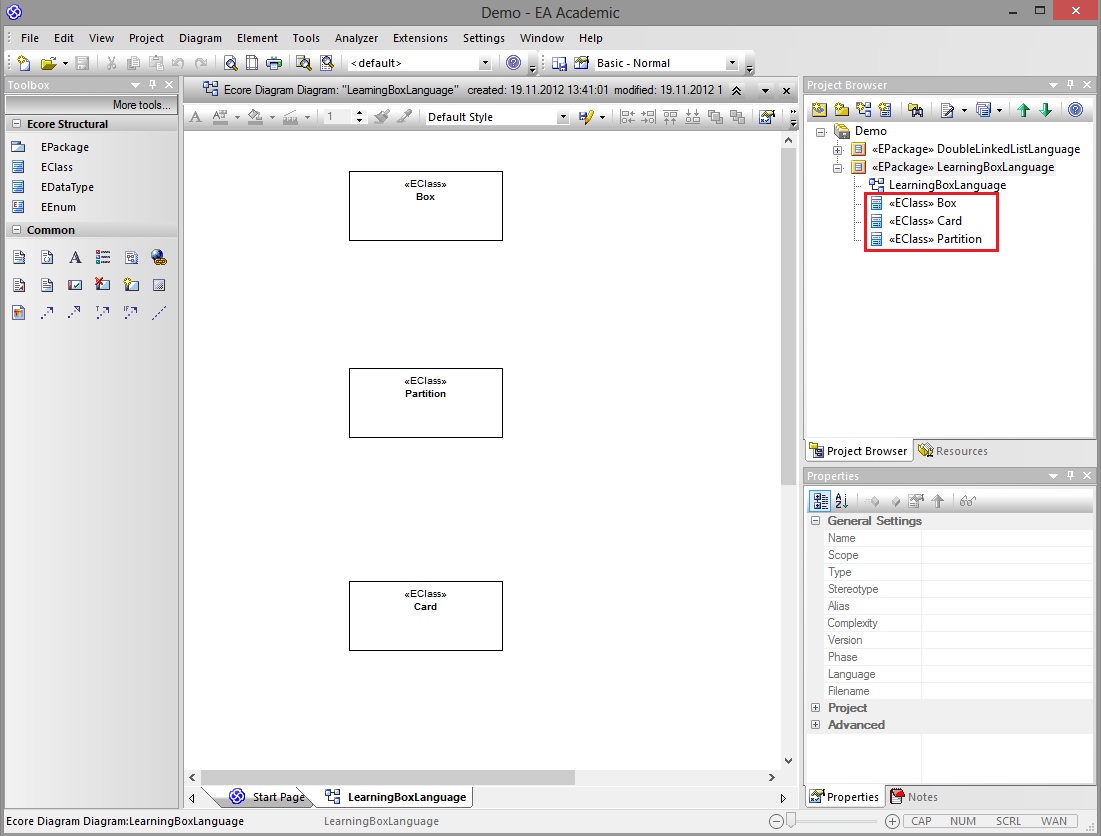
\includegraphics[width=0.9\textwidth]{ea_createPartitionCard}
	\caption{All EClasses for the metamodel}
	\label{ea:all_eclasses}
\end{figure}

\begin{figure}[htbp]
	\centering
  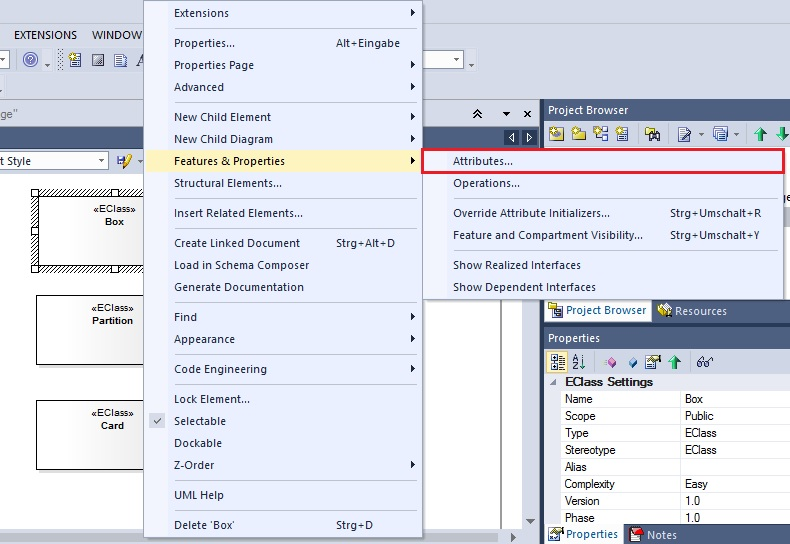
\includegraphics[width=0.7\textwidth]{ea_contextAddAttribute}
	\caption{Context menu for an EClass}
	\label{ea:attribute}
\end{figure}
\FloatBarrier

\item[$\blacktriangleright$] Enter \texttt{name} as the name of the attribute, select \texttt{EString} as its type from the drop-down menu, and press
\texttt{Save} (Fig.~\ref{ea:attribute_properties}). New attributes for the same EClass can be added by pressing \texttt{New}.

\vspace{1.0cm}

\begin{figure}[htbp]
	\centering
  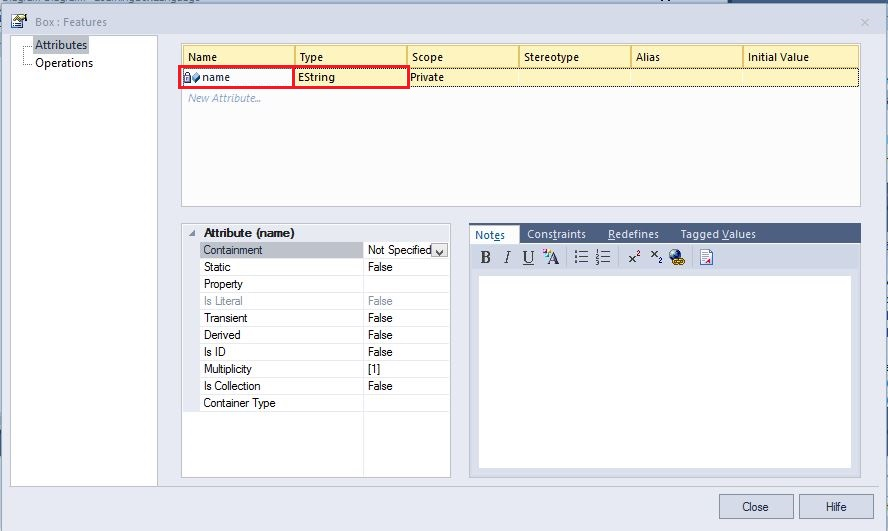
\includegraphics[width=0.9\textwidth]{ea_addAttributesDialogue}
	\caption{Adding attributes to an EClass}
	\label{ea:attribute_properties}
\end{figure}

\vspace{0.5cm}

\item[$\blacktriangleright$] Add the remaining attributes analogously to each EClass until your workspace resembles Fig.~\ref{ea:attribute_completed}.

\vspace{0.5cm}

\item[$\blacktriangleright$] Save and export to Eclipse. After refreshing your workspace, your \texttt{.ecore} model can now be expanded as it includes
every class and attribute from your metamodel. So far, so good!

\newpage

\vspace*{3cm}

\jumpSingle{static:references splash}

\begin{figure}[htbp]
	\centering
  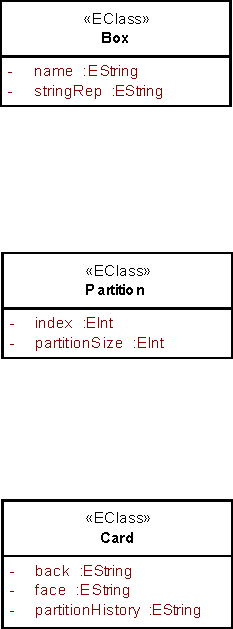
\includegraphics[width=0.35\textwidth]{ea_allAttributes}
	\caption{Main EClasses declared with their attributes}
	\label{ea:attribute_completed}
\end{figure}
\FloatBarrier

\end{itemize}
